%% IDE has R L T A 3
%% timetable has L R A 3 - pretty much the order of the 2009 examples.tex
% TODO for future: check taht loop demos, etc, use ":" rather than ","
% for string concatenation

\documentclass[12pt,a4paper,twoside]{article}
\usepackage{graphicx,fancyhdr}

\setlength{\parindent}{0cm}
\setlength{\parskip}{2ex plus1ex minus 0.5ex}

\addtolength{\evensidemargin}{-2.5cm}
\addtolength{\oddsidemargin}{-0.5cm}
\addtolength{\textwidth}{3cm}

\addtolength{\headheight}{0.2cm}
\addtolength{\topmargin}{-2.5cm}
\addtolength{\textheight}{2.5cm}

% \newcommand{\source}[1]{\textbf{\verb^#1^}}}
\renewcommand{\_}{\texttt{\symbol{95}}}
\addtolength{\fboxsep}{0.1cm}
\newcommand{\param}[1]{\textit{\textrm{\textmd{#1}}}}
\newcommand{\codebar}{\rule{\textwidth}{0.3mm}}
\newcommand{\todo}{\textbf{TODO}}

\newlength{\codelen}
\newcommand{\code}[1]
{\begin{center}\fbox{\parbox{16cm}{\texttt{#1}}}\end{center}}

\newcommand{\mission}[1]{\item[#1:]}
% \newcommand{\mission}[1]{\texttt{#1}\hspace{3mm}}

\fancyhead{}
\fancyhead[RO,LE]{\thepage}
\fancyhead[LO,RE]{ROBOC Summer School User Manual}
\fancyfoot{}
\pagestyle{fancy}
% \pagestyle{empty}

\setcounter{secnumdepth}{1}

\newenvironment{bulletlist}
{
	\begin{itemize}
	\addtolength{\itemsep}{-1mm}
	% \setlength{\itemsep}{0ex}
	\setlength{\parsep}{0ex}
}
{
	\end{itemize}
}

\newenvironment{alphalist}
{
	\begin{enumerate}
	\setlength{\itemsep}{0ex}
	\setlength{\parsep}{0ex}
	\renewcommand{\labelenumi}{(\alph{enumi})}
}
{
	\end{enumerate}
}

\newenvironment{numericlist}
{
	\begin{enumerate}
	\addtolength{\itemsep}{-1mm}
	% \setlength{\itemsep}{0ex}
	\setlength{\parsep}{0ex}
}
{
	\end{enumerate}
}

\usepackage{hyperref}
\begin{document}

\centerline{\textbf{\LARGE ROBOC Summer School User Manual}}
\vspace{0.5cm}
\centerline{August 2010}
\centerline{Author: David Ingram}
\centerline{Revised: David Eyers (\texttt{David.Eyers@cl.cam.ac.uk})}

{ \parskip 1mm plus 1pt \tableofcontents }

\newpage
\section{Usage}

Here is the editor screen (the program names (e.g.\ SKETCH) will probably be different
from yours):

\begin{center}
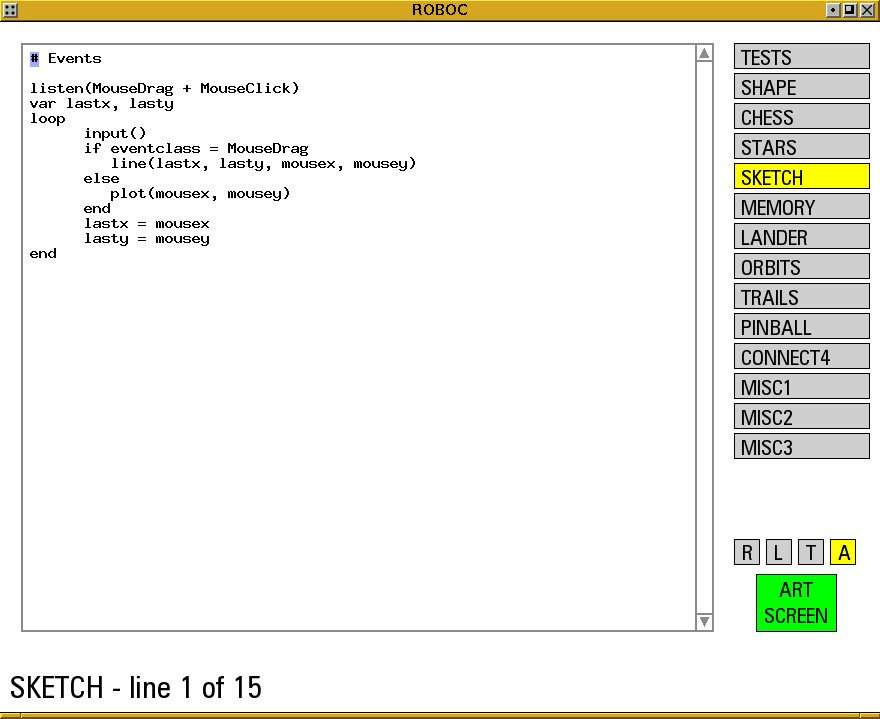
\includegraphics[scale=0.6,angle=0]{screenshots/ide/editor}
\end{center}

The wide grey buttons on the right switch between different slots. Each
slot can store one program. The currently selected slot is highlighted
in yellow. If there are more slots than can be
displayed in one go, scroll arrows will appear at the bottom of the
slot list.

\subsection{The editor}

You can type the program into
the main text area. Navigate with the \textbf{arrow}, \textbf{pgup},
\textbf{pgdn}, \textbf{home} and \textbf{end} keys. If the
current program is too long to fit on the screen you can also use the
scrollbar to move to different parts of it.
Erase with the \textbf{backspace} and \textbf{delete} keys.
Press the \textbf{tab} as appropriate
to indent your program (this is unnecessary when the automatic indent
option is
turned on).

\subsection{Clipboard functions}

You can select text in the editor by holding down the \textbf{shift key}
and pressing the cursor keys. The selected text is highlighted in
orange. You can also select the whole of the current program by
pressing \textbf{ctrl-a}.
Once text has been highlighted you can cut/copy/paste it with
\textbf{ctrl-x/c/v}.
It is possible to copy
text from one slot, change slots, then paste it into another program.
This is a good way to start a new program---you can copy one you
already have and then modify it to do something different.

\subsection{Editor options}

The bottom right of the status line shows options for case sensitivity
and for indentation. Press \textbf{both shift keys} together to
toggle case sensitivity on and off (by default it is off). Press
\textbf{shift-tab} to toggle indentation between normal and fully
automatic (the default is fully automatic).

\subsection{Switching to the output screen}

If you press the large green ``Screen'' button, you will
be taken to a screen like this one:

\begin{center}
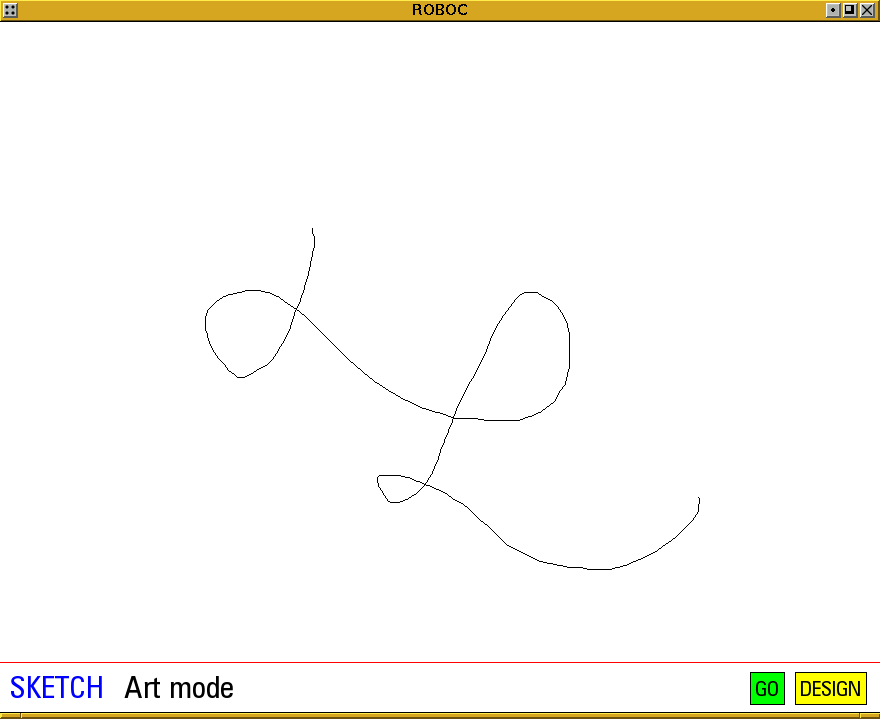
\includegraphics[scale=0.6,angle=0]{screenshots/ide/art_screen}
\end{center}

From here the ``Go'' button actually runs the program that you were
just looking at in the editor screen.
The ``Design'' button takes you back to the editor screen.
These two buttons disappear whilst
the program is running (press the \textbf{escape} key if you need to stop
the program part way through).

\subsection{Modes}

To change mode, make sure you are in the editor, then press one of the
small buttons marked `R', `L', `T', `A', and `3' in the bottom right
corner of the screen. The modes are as follows:

\begin{tabular}{|l|l|l|}
\hline
Small button & Mode name & Manual page \\
\hline
\textbf{T} & Text & \pageref{sec:text-mode} \\ 
\textbf{A} & Art & \pageref{sec:art-mode}\\ 
\textbf{L} & Logo & \pageref{sec:logo-mode}\\
\textbf{R} & Robot & \pageref{sec:robot-mode}\\
\textbf{3} & 3D & \pageref{sec:3d-mode}\\
\hline
\end{tabular}

A number of language features are available in all modes, but are
explained in the context of a particular mode in this manual.
\begin{itemize}
\item Details of the standard math library are on page \pageref{sec:stand-math-libr}
\item The string library functions are described on page \pageref{sec:string-libr-funct} 
\item Networking functions are explained on page \pageref{sec:networking-functions}
\end{itemize}

\subsection{Errors and Debugging}

It is \emph{very} easy to make mistakes when writing programs---most
people need a couple of tries before they get them right.
If there is a mistake in your program that prevents the computer
from understanding it, the program will stop and you will be
taken back to the editor screen. The line where the computer thinks
the mistake is will be highlighted in red. Look at the bottom of
the screen for a message that may help to explain what is wrong
with it. You should correct the mistake, then switch back to the
output screen to try running it again. Ask for help if you are still
stuck and can't see what the problem is.

\subsection{Keyboard shortcuts}

\begin{tabular}{|l|l|}
\hline
\textbf{ctrl-up/down} & change slot \\
\textbf{ctrl-left/right} & change mode \\
\textbf{insert} & switch to the output screen \\
\hline
\textbf{return} & ``go'' when on the output screen\\
\textbf{escape} & stops the program \\
\textbf{space} & switches back to the editor screen\\
\hline
\end{tabular}


\newpage
\section{The \textbf{\texttt{roboc}} Language}

\subsection{Layout}

\begin{bulletlist}
\item One statement per line
\item Blank lines, indentation and spaces are ignored by the interpreter
\item Indentation helps human readers, however%---you should always try
%  to make your programs as human-readable as possible!
\end{bulletlist}

\subsection{Comments}

\begin{bulletlist}
\item Comments start with the \verb^#^ character and continue until the end
      of the line
\end{bulletlist}

\subsection{Keywords}

There are 9 keywords. They must be entered in lower case:

{\bfseries \ttfamily
\begin{tabular}{|lllllllll|}
\hline
var & fn & return & if & else & elif & while & loop & end\\
\hline
\end{tabular}
}

The program starts with the first command that is not a function
definition

\subsection{Variables}

\begin{bulletlist}
\item Variables consist of global variables, function parameters,
	loop counter variables and local variables
\item Globals and locals may be declared with the \verb^var^
   statement before their first use
\item Loop counter variables are implicitly defined by the \verb^loop^
	instruction, and function parameters by the function definition
\item The \verb^var^ statement can optionally initialise each value
\item The \verb^var^ statement can be omitted, in which case variables
   are declared implicitly by assignment to them
\item The \verb^var^ statement cannot be omitted for arrays or for local
	variables with the same name as a global variable
\item The \verb^var^ statement can declare (and initialise) several
	variables on one line, separated by commas
\item Any variable may hold either an integer, a number or some text
\item Data types are not declared and all variables are named in the same way
\end{bulletlist}

Example:
\begin{verbatim}
var speed = 0, dx, dy, lives = 3
\end{verbatim}

\subsection{Text strings}

\begin{bulletlist}
\item String constants appear in double quotes
\item Strings may be compared for equality or lexicographic ordering
	using the normal comparison statements
\item Strings may be joined with the \verb^;^ or \verb^:^ operators
\item The \verb^:^ operator inserts an extra space
\item Integers and other numbers are automatically converted to text
	when required
\item A text string which represents a number is automatically
	narrowed to one of the numeric types internally when the value is set
\end{bulletlist}

Example:
\begin{verbatim}
a = "foo"
b = "bar"
c = a ; b
\end{verbatim}

\subsection{Expressions}

\begin{bulletlist}
\item The five arithmetic operators are \verb^+ - * / %^ (add,
	subtract, multiply, divide and remainder)
\item Division may create fractions, e.g. \verb^5 / 2 = 2.5^
\item Remainder works with whole numbers, e.g. \verb^20 % 9 = 2^
\item The \verb^* /^ and \verb^%^ operators have higher precedence
                               (i.e.\ order of operations) than
	\verb^+^ and \verb^-^ (the first three kinds are evaluated first)
\item The \verb^;^ and \verb^:^ operators have lower precedence than
	all the arithmetic operators
\item Operators of equal precedence are always evaluated left to right
\item Sub-expressions may be grouped with parentheses
\end{bulletlist}

Example:
\begin{verbatim}
speed = distance / (stop - start)
\end{verbatim}

\subsection{Conditional (\texttt{if}) statements}

\begin{bulletlist}
\item \verb^if^ statements are used to make decisions within a program
\item Comparisons can only occur in \verb^if^ statements
\item The four comparison operators are \verb^< > = ~^
\item \verb^~^ means ``not equal''
\item The special values \verb^true^ and \verb^false^ are allowed
      instead of a comparison
\item Comparisons can be chained together with \verb^and^ and \verb^or^
\item \verb^if^ blocks are terminated by the \verb^end^ keyword
\item There are optional \verb^else^ and \verb^elif^ blocks
\end{bulletlist}

Examples:
\begin{verbatim}
if lives = 0
   end_game()
end

if item = Door and keys ~ 0
   next_level()
elif monster_distance() < 2
   lives = lives - 1
end
\end{verbatim}

\subsection{Loops}

\begin{bulletlist}
\item Loops are a way to repeat the same set of actions
\item There are two styles of loop construct; if time is limited
	typically only one style is introduced. The new style is similar to
	``for'' loops and easier to use
\item \textit{Old-style loops:} \verb^while^ loops repeat as long as
	the condition is true
\item \textit{New-style loops:} \verb^loop^ increments a counter variable
	from a start to a finish value
\item \verb^loop^ on its own starts an infinite loop
\item \verb^while^ and \verb^loop^ blocks are terminated by the \verb^end^
	keyword
\end{bulletlist}

Examples:
\begin{verbatim}
n = 1
while n < 11
   print n, " squared is ", n * n
   n = n + 1
end

while true
   print "forever"
end

loop n from 1 to 10
   print n, " squared is ", n * n
end

loop
   print "forever"
end
\end{verbatim}

\subsection{Functions}

\begin{bulletlist}
\item Functions may be defined with the \verb^fn^ keyword
\item Functions definitions finish with the \verb^end^ keyword
\item Functions may not be defined inside other functions
\item Functions may take any number of parameters
\item Functions may return a single result
\item At run-time functions may call each other recursively
\item Parameters are separated by commas and listed in parentheses
\item The parentheses on function definition lines are optional
\item The parentheses for function calls are optional if
	\begin{bulletlist}
	\item The function takes no arguments, or
	\item The function call is on a line by itself
	\end{bulletlist}
\end{bulletlist}

Example:
\begin{verbatim}
factorise(100)

fn factorise(n)
   loop i from 2 to sqrt(n)
      if n % i = 0
         print i
         factorise(n / i)
         return
      end
   end
   print n
end
\end{verbatim}

\subsection{Arrays}

\begin{bulletlist}
\item Arrays must be declared with a \verb^var^ statement
\item Arrays may be local or global
\item Array items are accessed with square brackets
\item Arrays are 1-dimensional, with indices from $0$ to $n - 1$
\item Arrays may be passed as arguments by reference (i.e.\ the one
  instance of the array will be shared between function caller and callee)
\item The special index \verb^#^ gives the array size
\end{bulletlist}

Example:
\begin{verbatim}
var data[10]
data[0] = 1
data[1] = 1
fib(data)

fn fib(a[])
   loop i from 2 to a[#] - 1
      a[i] = a[i - 2] + a[i - 1]
   end
end
\end{verbatim}

\subsection{Output}

\begin{bulletlist}
\item \verb^print^ statements output a series of expression values and/or
      text messages to the screen
\item \textit{Deprecated:} you can \verb^print^ several things on the same
		line by separating them with commas (you should now use the colon
		and semi-colon operators to achieve this)
\end{bulletlist}

Example:
\begin{verbatim}
print "Score:" : points
\end{verbatim}

\subsection{Names}

\begin{bulletlist}
\item Names are strings of letters, numbers and underscores
\item Names may not contain other characters, such as spaces or punctuation
\item Names must not start with a number
\item Capitalisation does not matter, unless the case-sensitive option
	has been turned on
\item There are five uses for names:
	\begin{bulletlist}
	\item variables
	\item arrays
	\item keywords
	\item built-in functions
	\item user-defined functions
	\end{bulletlist}
	The same name cannot be used for more than one of these
	(e.g. a variable cannot have the same name as a function, etc)
\end{bulletlist}

\subsection{Comparison with the C language}

\begin{tabular}{|l|l|}
\hline
\rule[-2mm]{0mm}{6.5mm}
Roboc & C\\
\hline
One statement per line & Semicolons split statements \rule{0mm}{4.5mm}\\
\verb^end^ & Braces \verb^{ }^ delimit blocks\\
\verb^elif^ & \verb^else if^\\
\verb^=^ & \verb^==^ in tests\\
\verb^~^ & \verb^!=^\\
\verb^and or^ & \verb^&& ||^\\
\verb^loop^ & \verb^for^\\
Built-in graphics & Libraries\\
Interpreted & Compiled \rule[-3mm]{0mm}{3mm}\\
\hline
\end{tabular}

Other differences are that C requires parentheses around conditions and
loop parameters, but does not use \verb^fn^ when defining functions.

Extra features in C, not found in roboc:

\begin{tabular}{l@{\hspace{10mm}}l}
Static data types & More tests: \verb^<= >=^\\
Pointers & A logical `not' operator\\
More operators: \verb^& | ++ -- += *= -= /=^\\
\end{tabular}

\newpage
\section{3D Mode} \label{sec:3d-mode}

In 3D mode the display shows a large arena, with some raised platforms
for constructing objects.
%\subsection*{Co-ordinates and axes}
The origin (of the coordinate space) is in the centre, 5 metres above the middle platform.
The x axis points `east', the y axis points `north', and the z axis
points directly upwards.

%\section*{Functions}
%
%\verb^scale(x, y, z)^ is an example of a \textit{function}.
%
%\begin{bulletlist}
%\item Functions in programming are different from functions in Maths
%\item Functions perform useful tasks, like drawing to the screen
%\item Many functions may have parameters (like x, y and colour),
%	which control exactly what they do
%\item Some functions calculate a result. These \textbf{are} like
%	Maths functions
%\end{bulletlist}

\subsection{Shapes}

The following functions draw shapes at the current position.
Unless transformed they generally have unit size.

\begin{verbatim}
cube()
sphere()
cylinder()
cone()
pyramid()
prism()
torus(thickness)
\end{verbatim}

The \verb^pyramid()^ is square-based. The \verb^prism()^ is right-angled
triangle-based.

The torus \verb^thickness^ parameter
must be greater than 0 and less than 1. A torus of thickness 1 would
have no hole in the middle, and one of thickness 0 would be thin enough to be
invisible.

\subsection{Transformations}

\begin{verbatim}
translate(x, y, z)
scale(x, y, z)
rotatex(angle)
rotatey(angle)
rotatez(angle)
colour(n)
mark()
recall()
\end{verbatim}

The three rotation functions rotate about the x, y or z axis respectively.\\
Positive rotations are clockwise about an axis, looking towards the origin.\\
Scale factors of more than 1 are enlargements; factors less than 1 make
objects smaller.

%\verb^mark()^ and \verb^recall()^ save position, orientation,
%scaling factors and drawing colour. They may be nested as long as
%every \verb^mark()^ has one matching \verb^recall()^.

3D mode uses the same colour names and numbers as Art mode (see page \pageref{roboc:colours}).
%\subsection*{Colour}
%
%\begin{verbatim}
%colour(name)
%\end{verbatim}
%
%The following colour names can be used:
%
%\begin{verbatim}
%White   Red      Yellow   Sky    Grey    Purple
%Black   Orange   Green    Blue   Brown   Pink
%\end{verbatim}
%

\subsubsection*{Order of transformations}

Transformations move around the world from the origin in order.\\
The effect they have on a particular object is in \textbf{reverse} order.\\

\subsubsection*{Scope of transformations}

Each transformation effects \textbf{every} object that is drawn after
that point, not just the next one!\\
This is useful to scale or rotate a complete model.\\
The disadvantage is you must undo transformations to get back to where
you started.\\

\subsection{Remembering positions}

\begin{verbatim}
mark()
recall()
\end{verbatim}

\verb^mark()^ and \verb^recall()^ save position, orientation,
scaling factors and drawing colour. They may be nested as long as
every \verb^mark()^ has one matching \verb^recall()^.\\

%E.g. house and windows.

\subsection{Global status variables}

The following three variables always contain the position of the camera:

\begin{verbatim}
playerx
playery
playerz
\end{verbatim}

\subsection{Viewer controls (centred mode)}

The camera always faces towards the origin in centred mode,
but you can change its position in the room using the following keys:

\begin{tabular}{ll}
Cursor left  & Rotate camera left\\
Cursor right & Rotate camera right\\
Cursor up    & Zoom in towards the centre of the room\\
Cursor down  & Zoom out away from the centre of the room\\
J            & Jet-pack (release for normal gravity)\\
W            & Switch to walk mode\\
Escape       & Back to the editor screen\\
\end{tabular}

\subsection{Viewer controls (walk mode)}

In this mode you can move around the arena freely.

\begin{tabular}{ll}
Cursor left  & Turn left\\
Cursor right & Turn right\\
Shift-Cursor left  & Side step left\\
Shift-Cursor right & Side step right\\
Cursor up    & Walk forward\\
Cursor down  & Walk backward\\
Shift-Cursor up & Look upwards\\
Shift-Cursor down & Look downwards\\
Enter        & Look horizontally\\
J            & Jet-pack (release for normal gravity)\\
C            & Switch to centred mode\\
Escape       & Back to the editor screen\\
\end{tabular}

\newpage
\section{Logo Mode} \label{sec:logo-mode}

In logo mode the roboc program controls a turtle that paints
a line as it moves around on the screen. The turtle itself is
not shown and the output screen is initially blank.

\subsection{Turtle control}

\begin{bulletlist}
\item \verb^turn^ and \verb^move^ control the turtle
\item Angles are measured clockwise in degrees
\end{bulletlist}

For example:
\begin{verbatim}
turn 45
move 100
turn -90
\end{verbatim}

\subsection{Setting the starting position}

\verb^origin(^\emph{position}\verb^)^

Where \emph{position} is one of:
\begin{verbatim}
TopLeft      Top      TopRight
Left         Centre   Right
BottomLeft   Bottom   BottomRight
\end{verbatim}

\newpage
\section{Robot Mode} \label{sec:robot-mode}

In robot mode the aim is to steer a small robot around different
environments, navigating around walls and collecting objectives. The
objectives are always called ``Fruit'' although on some missions they
take the form of diamonds, footprints, fuel canisters and so on.

\begin{center}
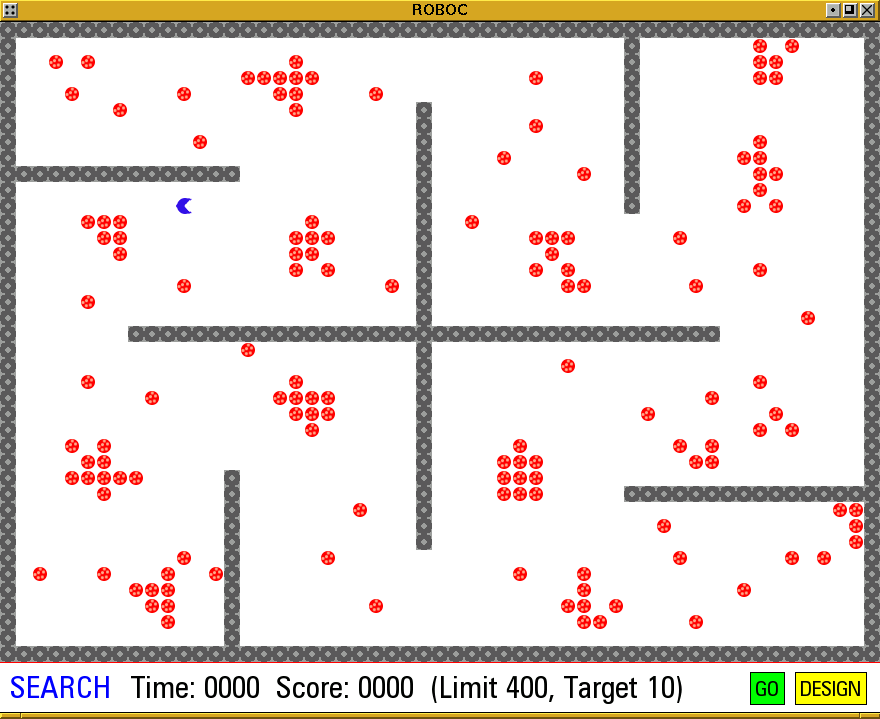
\includegraphics[scale=0.6,angle=0]{screenshots/robot/search}
\end{center}

\subsection{Movement}

In robot mode, you use the \verb^move^ and \verb^turn^
keywords to control the robot. Here are some examples:

\begin{verbatim}
turn -1
move
turn 1
move
turn 2
\end{verbatim}

\begin{bulletlist}
\item In robot mode, the \verb^move^ command is used without a
	parameter, and always moves a single space forward.
\item The robot is steered with \verb^turn^ commands. 
	The angle to turn is measured in right angles (not degrees),
	so \texttt{turn 1} turns 90 degrees to the right.
\item Negative turns are to the left
\end{bulletlist}

Here's a loop for moving more than one square
in a straight line:

\begin{verbatim}
loop n from 1 to distance
   move
end
\end{verbatim}

\subsection{Senses}

There are five functions you can use to sense objects in the proximity
of the robot:

\begin{verbatim}
thing = touch()
thing = leftside()
thing = rightside()
thing = look()
count = smell(thing)
\end{verbatim}

\begin{bulletlist}
\item \texttt{thing} will be one of:
	\texttt{Floor}, \texttt{Wall} or \texttt{Fruit}

\item \texttt{touch()} examines the square directly in front of the
	robot, \texttt{leftside()} looks at the square immediately to its
	left and \texttt{rightside()} looks at the square to its right.

\item \texttt{look()} looks forward in a straight line to the first
	non-empty square, however distant that might be.

\item \texttt{smell(thing)} counts how many of \texttt{thing} are present
	in the 5x5 square portion of the grid centred on the robot.
\end{bulletlist}

Examples:

\verb^if touch() = Wall^\\
\verb^   ^\textit{Do something}\\
\verb^end^\\
\verb^if leftside() = Fruit^\\
\verb^   ^\textit{Do something}\\
\verb^end^\\
\verb^if rightside() ~ Wall^\\
\verb^   ^\textit{Do something}\\
\verb^end^\\
\verb^if look() = Fruit^\\
\verb^   ^\textit{Do something}\\
\verb^end^\\
\verb^if smell(Fruit) > 2^\\
\verb^   ^\textit{Do something}\\
\verb^end^\\

\subsection{Usage instructions}

\textbf{Controls:}
Press the \textbf{shift} key to speed up time. Press \textbf{escape} to abort.

\textbf{Time:}
The robot has a time limit set by the mission (for example, 400).
This is the number of time steps in which it must collect as much fruit
as possible. Any move or turn command takes one time step.

Calculations take no time provided your program doesn't
execute more that 250 lines of code between each move/turn.
Exceeding that limit costs you another time step.

\textbf{Scoring:}
Your robot scores 1 point per piece of fruit collected. 

\textbf{High scores:}
Your best score appears as a number next to the name of each mission
in the editor screen.

\textbf{Target score:}
Every mission has a target score. You should try to reach this.
The target score isn't the highest possible on most missions, but
if you get it you know you have reached a good standard. When you have
achieved the target your score for that mission will turn from red to green.

\newpage
\section{Text Mode} \label{sec:text-mode}

In text mode, the output screen displays the messages from \verb^print^
statements. It will scroll if the output reaches the bottom of the screen.
Note that currently there is no way to scroll back up to see previous output.

\subsection{Standard math library} \label{sec:stand-math-libr}

These functions are all available in all modes (not just text mode),
with the exception of \verb^random()^, which is not available in
robot mode.

\begin{verbatim}
y = sin(x)
y = cos(x)
y = tan(x)
y = sqrt(x)
y = pow(x, exponent)
y = ln(x)
n = round(x)
n = random(from, to)
\end{verbatim}

The \verb^sin^, \verb^cos^ and \verb^tan^ functions all accept
arguments in degrees.

One variable is predefined:

\begin{verbatim}
Pi
\end{verbatim}

\subsection{String library functions} \label{sec:string-libr-funct} 

These functions are also available in all modes:

\begin{verbatim}
letters(string)
words(string)
substring(first, last, string)
word(n, string)
\end{verbatim}

\verb^letters()^ and \verb^words()^ count the number of characters
and words in a string. Words are anything separated by spaces.
\verb^word()^ returns the \verb^n^th word in a string. Words and
characters are labelled starting from zero.

The following function is available in all modes except for robot
mode or 3D mode:

\begin{verbatim}
s = read()
\end{verbatim}

This inputs a line of text from the keyboard. In graphical modes or if
the IDE is running, the status line at the bottom of the screen is used
to accept input. In text mode without the IDE, the console is used instead.

\newpage
\section{Art Mode} \label{sec:art-mode}

Art mode provides a blank canvas on which the program can draw.

\subsection{Art mode colours}

\label{roboc:colours}
\begin{tabular}{|ll|ll|}
\hline
\rule{0mm}{4.5mm}%
0 & White   & 6  & Sky\\
1 & Black   & 7  & Blue\\
2 & Red     & 8  & Grey\\
3 & Orange  & 9  & Brown\\
4 & Yellow  & 10 & Purple\\
5 & Green   & 11 & Pink\\
\hline
\end{tabular}

% \subsection{Tile-based drawing functions}
% 
% The coordinate system origin is at the bottom left corner of the
% screen (mathematical coordinates, with $y$ increasing upwards).
% 
% \begin{verbatim}
% tile(x, y, colour)
% colour = inspect(x, y)
% \end{verbatim}
% 
% See the accompanying worksheet for examples and exercises using
% tile-based drawing.
% 
% Non-absolute position drawing:
% \verb^move^ and \verb^turn^-based drawing:
% 
% \begin{verbatim}
% teleport(x, y)
% paint(colour)
% \end{verbatim}

\subsection{Pixel-based drawing functions}

The coordinate system origin is at the top left corner of the
screen (graphics coordinates, with $y$ increasing downwards).

\begin{verbatim}
plot(x, y)
ink(colour)
colour = examine(x, y)
line(x1, y1, x2, y2)
spot(x, y, radius)
circle(x, y, radius)
box(x, y, width, height)
image(x, y, object)
icon(x, y, object)
background(name)
cursor(x, y)
\end{verbatim}

\verb^ink^ changes the current colour used by all the drawing
functions. \\
%except \verb^tile^ above.\\
\verb^plot^ paints one pixel.\\
\verb^spot^ draws a filled circle and \verb^box^ draws a filled rectangle.\\
\verb^image^ paints one of the built-in images, listed on page
	\pageref{images}.\\
\verb^icon^ is the same as \verb^image^, but reduces it to half size.\\
\verb^background^ draws one of the supplied full-screen pre-rendered images,
	listed on page \pageref{backgrounds}.\\

In art mode, text output with the \verb^print^ statement appears on the
canvas, at the last position set with the \verb^cursor^ function.
The screen does not scroll.

\subsection{Constants}

\begin{verbatim}
ScreenWidth
ScreenHeight
\end{verbatim}

\subsection{Art mode input}

Functions:

\begin{verbatim}
listen(events)
class = input()
class = poll()
\end{verbatim}

\verb^listen^ specifies which kinds of event the program should respond to.
\verb^input^ waits for the next event; \verb^poll^ reports an event
if one has already taken place but returns \verb^0^ immediately otherwise.
After an event has occurred you can inspect the global status variables
below to find out what it was.

Event class constants:

\begin{verbatim}
MouseClick
MouseDrag
MouseRelease
KeyPress
KeyRelease
\end{verbatim}

Global status variables set by \verb^input()^ and \verb^poll()^:

\begin{verbatim}
mousex
mousey
mousebutton
keyval
mousedx
mousedy
eventclass
\end{verbatim}

Tile-based status variables---also set by \verb^input()^ and \verb^poll()^:

\begin{verbatim}
pointerx
pointery
\end{verbatim}

These are like \verb^mousex^ and \verb^mousey^ but report position in
the tile co-ordinate system rather than in pixels.

\subsection{Networking functions} \label{sec:networking-functions}

Networking is available in all modes (not just art mode), provided the
person who installed ROBOC has started the network server.
Incoming messages generate events.

The networking functions are:

\begin{verbatim}
self(string)
send(name, message)
\end{verbatim}

The network event class constant is:

\begin{verbatim}
NetEvent
\end{verbatim}

The global status variable set by \verb^input()^ and \verb^poll()^ is:

\begin{verbatim}
message
\end{verbatim}

\subsection{Art mode time functions}

These are useful for animations:

\begin{verbatim}
delay(microseconds)
microseconds = time()
\end{verbatim}

\newpage
\subsection{Art mode keys}

These are the key values stored in \verb^keyval^.
Values up to 127 are standard ASCII.
128 to 133 are roboc extensions.

\begin{verbatim}
 33   !     65    A      97   a     48    0
 34   "     66    B      98   b     49    1
 35   #     67    C      99   c     50    2
 36   $     68    D     100   d     51    3
 37   %     69    E     101   e     52    4
 38   &     70    F     102   f     53    5
 39   '     71    G     103   g     54    6
 40   (     72    H     104   h     55    7
 41   )     73    I     105   i     56    8
 42   *     74    J     106   j     57    9
 43   +     75    K     107   k      8    Backspace
 44   ,     76    L     108   l      9    Tab
 45   -     77    M     109   m     10    Newline
 46   .     78    N     110   n     13    Return
 47   /     79    O     111   o     27    Escape
 58   :     80    P     112   p    127    Delete
 59   ;     81    Q     113   q     32    Space
 60   <     82    R     114   r    132    Left shift
 61   =     83    S     115   s    133    Right shift
 62   >     84    T     116   t    128    Cursor left
 63   ?     85    U     117   u    129    Cursor right
 64   @     86    V     118   v    130    Cursor up
 91   [     87    W     119   w    131    Cursor down
 92   \     88    X     120   x
 93   ]     89    Y     121   y
 94   ^     90    Z     122   z
 95   _
 96   `
123   {
124   |
125   }
126   ~
\end{verbatim}

\subsection{Background images}
\label{backgrounds}

The following full-screen (880 by 640 pixel) images are supplied:
\begin{verbatim}
dragon   capricorn   track
\end{verbatim}

\newpage
\subsection{Art mode images}

These are used with the pixel-based \verb^image()^ function.

\label{images}

\begin{tabular}{|ll|ll|ll|ll|}
\hline
\rule{0mm}{4.5mm}%
  0 & Ant         & 26 & Apple      & 52 & Beachball       &  82 & Music\\
  1 & Bear        & 27 & Bananas    & 53 & BlackBalloon    &  83 & OrangeBalloon\\
  2 & Butterfly   & 28 & Beer       & 54 & BlueBalloon     &  84 & Paintbrush\\
  3 & Cat         & 29 & Burger     & 55 & Boat            &  85 & Palette\\
  4 & Diplodocus  & 30 & Cake       & 56 & Bomb            &  86 & PaperDart\\
  5 & Dog         & 31 & CandyCane  & 57 & Boy             &  87 & Pencil\\
  6 & Dolphin     & 32 & Carrot     & 58 & Card            &  88 & PinkBalloon\\
  7 & Dove        & 33 & Cheese     & 59 & Clock           &  89 & PirateFlag\\
  8 & Elephant    & 34 & Cherries   & 60 & Clover          &  90 & Pumpkin\\
  9 & Fish1       & 35 & Coffee     & 61 & Cog             &  91 & RedBalloon\\
 10 & Fish2       & 36 & Croissant  & 62 & Compass         &  92 & RedLight\\
 11 & Frog        & 37 & Fries      & 63 & Daffodil        &  93 & Roller\\
 12 & Horse       & 38 & Glass      & 64 & Dice            &  94 & Scissors\\
 13 & Ladybird    & 39 & Grapes     & 65 & Drums           &  95 & Scroll\\
 14 & Lion        & 40 & IceCream   & 66 & Flowers         &  96 & Snowman\\
 15 & Lobster     & 41 & Lemon      & 67 & Football        &  97 & SuitClubs\\
 16 & Penguin     & 42 & Orange     & 68 & Girl            &  98 & SuitDiamonds\\
 17 & Pterodactyl & 43 & Peach      & 69 & GreenBalloon    &  99 & SuitHearts\\
 18 & Puffin      & 44 & Pie        & 70 & GreenLight      & 100 & SuitSpades\\
 19 & Seagull     & 45 & Pineapple  & 71 & Harp            & 101 & Sword\\
 20 & Seal        & 46 & Pizza      & 72 & Heart           & 102 & TeddyBear\\
 21 & Sheep       & 47 & Sandwich   & 73 & HotAirBalloon   & 103 & Tools\\
 22 & Siamese     & 48 & Strawberry & 74 & Hourglass       & 104 & Tulips\\
 23 & Stegosaurus & 49 & Tea        & 75 & Lamp            & 105 & Unlocked\\
 24 & Swan        & 50 & Watermelon & 76 & Leaf            & 106 & WhiteBalloon\\
 25 & Tiger       & 51 & Wine       & 77 & Locked          & 107 & WhiteFlower\\
    &             &    &            & 78 & Luck            & 108 & Wigwam\\
    &             &    &            & 79 & MagicLamp       & 109 & YellowBalloon\\
    &             &    &            & 80 & MagnifyingGlass & 110 & YellowFlower\\
    &             &    &            & 81 & Mushroom        & 111 & YellowLight\\
\hline
\end{tabular}
\\[5mm]
If case sensitivity is switched off, which is the
default (\verb^Case: ANY^ appears in the IDE), these names must be referred
to with an initial underscore. For example, \verb^_Ant^ (or \verb^_ant^,
or \verb^_ANT^).
This is to prevent them clashing with your own variable names.
If case sensitivity is on (\verb^Case: SPEC^ appears in the IDE), the names
should be used without underscores, e.g. \verb^Ant^.

\appendix
\newpage
\section{The \textbf{\texttt{roboc}} Grammar}

\begin{verbatim}
<program> ::= <toplevel> <toplevel> ...
<toplevel> ::= <statement> | <fn-defn>
<fn-defn> ::= fn <fn-name> <formal-param>, <formal-param>, ... <NL> <block> |
   fn <fn-name> ( <formal-param>, <formal-param>, ... ) <NL> <block>
<formal-param> ::= <var> | <array-ref>
<stmt-list> ::= <statement> <statement> ...
<block> ::= <stmt-list> <end-stmt>
<end-stmt> ::= end <NL>
<statement> ::= <flow-of-ctrl> | <executable> <NL>

<flow-of-ctrl> ::= <return-stmt> <NL> | <if-construct> | <while-construct> |
   <loop-construct>
<return-stmt> ::= return | return <expr>
<if-construct> ::= if <cond> <NL> <stmt-list> <if-tail>
<if-tail> ::= <end-stmt> | else <NL> <block> |
   elif <cond> <NL> <stmt-list> <if-tail>
<while-construct> ::= while <cond> <NL> <block>
<loop-construct> ::= <loop-stmt> <NL> <block>
<loop-stmt> ::= loop <var> from <expr> to <expr> | loop

<cond> ::= <test> | <cond> and <test> | <cond> or <test>
<test> ::= <expr> <comparator> <expr> | true | false
<comparator> ::= < | > | = | ~

<executable> ::= <declaration> | <assignment> | <fn-call-stmt>
<declaration> ::= var <initializer>, <initializer>, ...
<initializer> ::= <var> | <var> = <expr> | <init-array>
<init-array> ::= <array-size>
<assignment> ::= <box> = <expr>
<box> ::= <var> | <array-element>
<fn-call-stmt> ::= <fn-call> | <fn-name> <actual-param>, <actual-param>, ...
<fn-call> ::= <fn-name> ( <actual-param>, <actual-param>, ... ) | <fn-name>
<actual-param> ::= <expr> | <array-ref>

<array-element> ::= <array> [ <expr> ]
<array-size> ::= <array> [ <expr> ]
<array-ref> ::= <array> [ ]

<expr> ::= <atomic> | <expr> <op> <atomic> | - <atomic>
<atomic> ::= <value> | <fn-call> | ( <expr> ) | <array-element> | <array> [ # ]
<op> ::= + | - | * | / | % | : | ;

<value> ::= <var> | <number> | <string>
<string> ::= " <char> <char> ... "
<char> ::= {Anything other than <NL> or "}
<comment> ::= # {Anything other than <NL>} ... <NL>

<var> ::= <name>
<array> ::= <name>
<fn-name> ::= <name>
<name> ::= <letter> <alphanum> <alphanum> ...
<alphanum> ::= <digit> | <letter>
<letter> ::= a | b | c | ... | y | z | A | B | C | ... | Y | Z | _

<number> ::= <integer> | <integer> <decimal>
<decimal> ::= . <integer>
<integer> ::= digit digit ...
<digit> ::= 0 | 1 | 2 | 3 | 4 | 5 | 6 | 7 | 8 | 9
\end{verbatim}

\end{document}
